\chapter{Experimenty}

\section{Ukážka vstupných dát ACN-Data}
\begin{figure}[H]
    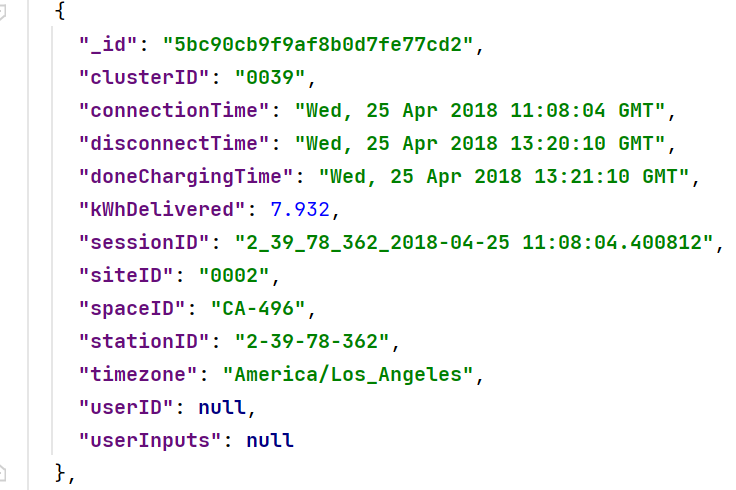
\includegraphics[width=0.8\textwidth]{images/acndata.png}
    \centering
    \caption[Ukážka vstupných dát ACN-Data]{Vstupné dáta z nabíjania jedného elektromobilu, ktorý prišiel na nabíjaciu stanicu 25. Apríla 2018. Zdroj: \cite{websiteacndata2023}.}
    \label{acndata:obr}
    \end{figure}
Obrázok vstupných dát \ref{acndata:obr} obsahuje viacero parametrov, ktoré používateľ musí zadať (napr kWhDelivered), aby mohol nabíjať svoj elektromobil na jednej staníc Caltech, JPL alebo Office001. Iné nabíjacie stanice používajú odlišné vstupné dáta, uvádza sa v \cite{lee2021adaptivephd}.

\section{Využité technológie}
V tejto sekcii spomíname technológie, na ktorých spočíva naša implementácia. Balíky popisujeme hlavne na základe informácií uvedených v ich README súboroch a na základe článku \cite{lee2021acnsim}. Podrobný návod, ako vytvoriť algoritmy na základe nasledujúcich balíkov sa nachádza v \cite{lee2021acnsim}.
\label{vychodiska:technologicke}

% TODO: nabijat len 8 amperov? skontrolovat!!!

\subsection{Balík acnportal.}
% \subsection{Balík acnportal.}
% \subsection{Balík acnportal}
Balík acnportal obsahuje záznamy nabíjania elektromobilov získane z nabíjacich stanic Caltech, JPL a Office001. Každý záznam nabíjania elektromobilu obsahuje jeho príchod, odchod a požadovanú energiu. Balík acnportal sa nachádza v \cite{acnportalrepository}. Balík acnportal pozostáva z viacerých komponentov:

\begin{enumerate}
    \item \textbf{ACN-Data}: Dáta získané z nabíjacích staníc pre elektromobily, konkrétne zo staníc Caltech, JPL a Office001. 
    Vodiči elektromobilov musia cez mobilnú aplikáciu zadať oskenovaný QR kód nabíjačky a potom zadať približný čas odchodu a množstvo požadovanej energie. 
    %Ak vodič neuvedie informácie cez mobilnú aplikáciu, nabíjačka bude nabíjať len 8 ampérov a ak ani po 15 minútach vodič neuvedie informácie, tak nabíjačka prestane nabíjať.  
    Dáta získané od vodičov elektromobilov, ale aj dáta slúžiace ku konfigurácii siete sú uložené v relačnej databáze. 
    Vďaka tejto úložnej vrstve vieme vytvárať vizualizácie pre vodičov elektromobilov a pre sieťových operátorov. 
    Ide hlavne o vizualizáciu stavu systému pre sieťových operátorov a stav nabíjania elektromobilov pre vodičov elektromobilov.
    \item \textbf{ACN-Sim}: ACN-Sim je simulátor používaný na testovanie a overovanie funkcionality algoritmov a systémov. Simulátor zabezpečuje realistické prostredie na overovanie funkcionality algoritmov, hlavne pre výskumníkov, ktorý nemajú prístup k reálnym nabíjacím systémom pre nabíjanie elektromobilov.
    \item \textbf{ACN-Live}: ACN-Live je hardvér, na ktorom bežia plánovacie algoritmy nabíjania elektromobilov v reálnom čase. Keďže má rovnaké rozhranie ako simulátor ACN-Sim, tak vieme testovať algoritmy implementované v ACN-Sim bez zmeny kódu. \cite{lee2021acnsim, lee2020adaptive}
\end{enumerate}

\begin{figure}[H]
    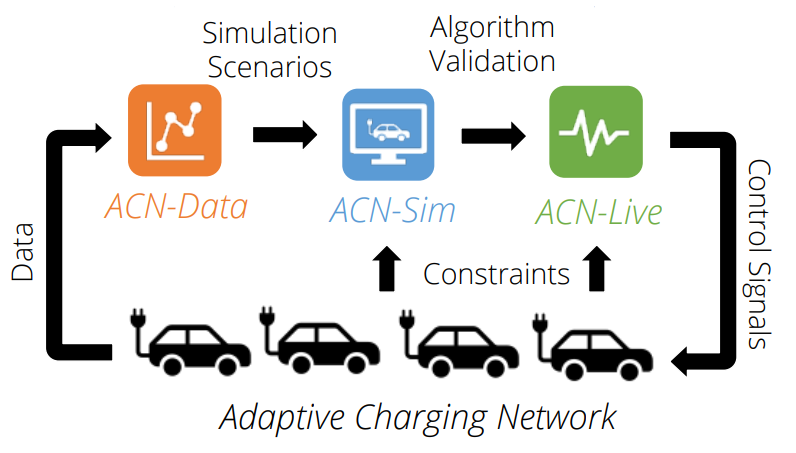
\includegraphics[width=0.8\textwidth]{images/acn_research_portal_pic.png}
    \centering
    \caption[Schéma acnportal.]{Schéma acnportal. Zdroj obrázka je \cite{lee2021acnsim}.}.
    \label{acn:obr}
    \end{figure}
Obrázok \ref{acn:obr} ilustruje interakciu medzi hlavnými komponentami acnportal. Dáta o nabíjaní získava komponent ACN-Data. O obmedzenia siete a validáciu algoritmov sa stará komponent ACN-Sim. V ACN-Live uvádzame konkrétne algoritmy z ACN-Sim do prevádzky. Na takú operáciu netreba meniť kód, lebo ACN-Sim a ACN-Live fungujú cez rovnaké rozhranie. \cite{lee2021acnsim,lee2021adaptivephd}

%TODO: overit vsetky napisane udaje, musi to sediet!




\subsection{Architektúra simulátora ACN-Sim}

\begin{figure}[H]
    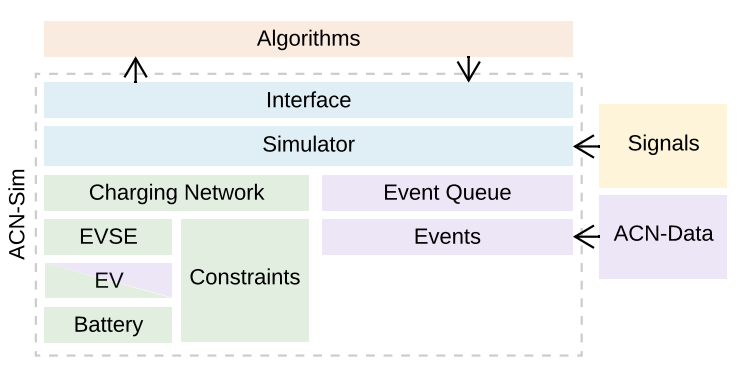
\includegraphics[width=0.8\textwidth]{images/acn_architecture.png}
    \centering
    \caption[Architektúra simulátora ACN-Sim.]{Architektúra simulátora ACN-Sim. Obrázok pochádza z článku \cite{lee2021acnsim}.}
    \label{architectureacnsim+:obr2}
    \end{figure}
Obrázok \ref{architectureacnsim+:obr2} popisuje architektúru simulátora ACN-Sim. Simulátor ACN-Sim má modulárnu, objektovo orientovanú architektúru. Pod každou krabicou v obrázku \ref{architectureacnsim+:obr2} chápeme základnú triedu, od ktorej môžu dediť nové triedy. Tieto nové triedy môžu napríklad obsahovať nové funkcie.  


Simulátor ACN-Sim obsahuje udalosti popisujúce príchod a odchod elektromobilov. Každá udalosť obsahuje informáciu, v ktorom časovom kroku behu simulátora sa má vykonať. V každom časovom kroku behu simulátora sa vykonávajú udalosti v predchádzajúcom časovom kroku alebo udalosti v aktuálnom časovom kroku. Po každej vykonanej udalosti sa spustí plánovací algoritmus a stav infraštruktúry sa aktualizuje. \cite{lee2021acnsim}


% \begin{figure}[H]
%     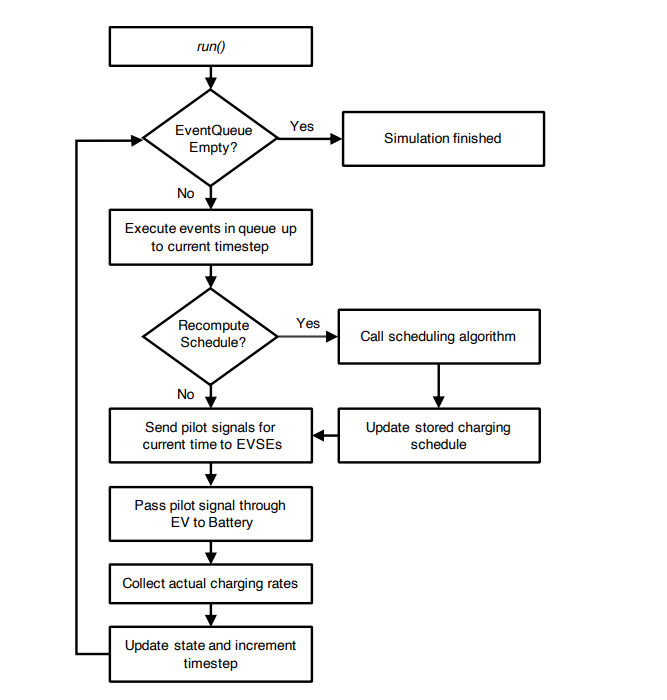
\includegraphics[width=0.8\textwidth]{images/simulator_run.png}
%     \centering
%     \caption[Vývojový diagram funkcie run() simulátora ACN-Sim.]{Vývojový diagram funkcie run() simulátora ACN-Sim. Obrázok pochádza z článku \cite{lee2021acnsim}.}
%     \label{architectureacnsim+:obr2}
%     \end{figure}

% \UNFIN

% nám pomáha pochopiť štruktúru a interakcie jednotlivých častí systému, aby sme vedeli implementovať vlastné algoritmy.


% \subsection{Interakcia medzi spotrebitelmi a smart grid}


%vsetky baliky sa zacinaju malym pismenom a su oddelene pomlckami

% TODO: blizsie popisat z coho pozostava ten balik!!!!
% namiesto repozitar balik napriklad!!
\subsection{Balík adacharge.}
% \subsection{Balík Adacharge}
Balík adacharge obsahuje kontrolný algoritmus MPC, ktorý je schopný riešiť viacero optimalizačných problémov v rámci plánovania nabíjania elektromobilov. Tento MPC algoritmus rieši aj problém, ktorý my riešime, a to problém pridelenia maximálnej energie elektromobilom pri zachovaní obmedzení infraštruktúry pomocou konvexnej optimalizácie. Podrobnejší popis a zdrojový kód balíka Adacharge sa nachádza v \cite{adachargerepository}.
% aj zaroven obmienat
\subsection{Balík acnportal-experiments.}
Balík acnportal-experiment obsahuje experimenty, ktoré využívajú balík acnportal. Tieto experimenty následne vedia zodpovedať výskumné otázky. Pre tvorbu nových experimentov, ktoré riešia náš problém sú podstatné experimenty 1.2 a 2.1. Tieto experimenty využívajú viacero plánovacích algoritmov a konfigurácii siete. Krátky popis experimentov:
\begin{enumerate}
    \item Experiment 1.2: Cieľom experimentu je porovnať viacero konfigurácii infraštruktúry siete a zároveň plánovacie algoritmy. Tento experiment poukazuje na výhody smart sietí. Jednou z výhod smart sietí je, že vedia riešiť problém dodania maximálneho množstva energie pri zachovaní obmedzení infraštruktúry siete.
    \item Experiment 2.1: Cieľom experimentu je porovnať výkonnosť týchto plánovacích algoritmov:  round robin,  earliest deadline first, least laxity first. Jedným z výsledkov experimentu je koľko percent požadovanej energie dodá elektromobilom každý algoritmus.
\end{enumerate}
%experiment 2.2 mozno pridat ale netyka sa toho co my riesime, riesi vykonnost planovacich algoritmov pri zmene modelu baterie atd





Podrobnejší popis a výsledky experimentov vieme nájsť v \cite{acnportalexperimentsrepository}.

%TODO: pojmy ako transformer vysvetlit alebo odstranit
%TODO: mozno pridat aj ten 3. experiment?
%TODO: pisat tie mena algoritmov jednotne
% \UNFIN

% \section{Aplikovateľnosť smart charging algoritmov.}

% Mnoho zaujímavých algoritmov z literatúry sa nedá využiť priamo v praxi. Hlavným dôvodom prečo sa nedajú aplikovať v praxi je poďla \cite{lee2021adaptivephd} to, že majú predpoklady, ktoré v praxi nefungujú alebo im chýba schopnosť splniť praktické obmedzenia a aj ciele.

% Uvádzame list vlastností smart changing algoritmu spomen , ktorý môže byť aplikovateľný v praxi:

% \begin{enumerate}
%     \item Algoritmy musia brať do úvahy používateľské vstupy ako napríklad čas odchodu a množstvo požadovanej energie.
%     \item Algoritmy musia vyriešiť jednoducho problém s viacerými cieľmi.
%     \item Algoritmy musia vedieť pracovať s obmedzeniami v niekoľkoúrovňovej nevyváženej infraštruktúry.
%     \item Výstup algoritmov (plán nabíjania) musí spĺňať aspoň jednu z týchto vlastností: plynulé nabíjanie alebo spravodlivé zdielanie kapacity medzi elektromobilmy.
%     \item Algoritmy musia byť odolné voči neistote v budúcich príchodoch elektromobilov. 
%     \item Algoritmy musia vedieť narábať s diskrétnymi bodmi pre pilotové signály.
%     \item Algoritmy musia mať schopnosť si nárokovať nevyužitú kapacitu v prípade, keď elektromobili nevyužívajú alokovaný pilotový signál. 
% \end{enumerate}

% Algoritmus, ktorý všetky tieto podmienky spĺňa sa nazýva Adaptive Scheduling  Algorithm (ASA). Podrobnejší popis, prečo tieto podmienky tento algoritmus spĺňa a aj list podmienok z ktorého sme čerpali sa nachádza v
% \cite{lee2021adaptivephd}.

% acnportalexperimentsrepository

% \subsection{Balík Acnportal-experiments}


% V tejto sekcii spomíname knižnice, frameworky a ďalšie technológie, ktoré sme pri implementácii použili.

% \subsection{Knižnica numpy}
% \label{ss:vych:techvych:numpy}
% Knižnica numpy rozširuje možnosti v oblasti práce s poľami. 
% V knižnici numpy sú 2 hlavné objekty: ndarray a ufunc. Pomocou objektu ndarray vieme definovať N-dimenzionálne pole a pomocou ufunc vieme definovať matematické funkcie. Každé pole objektu ndarray obsahuje homogénnu kolekciu prvkov.
% % Tie sa v štruktúre s bežnými poľami neodlišujú, to znamená že prvý prvok poľa má index 0 a posledný $n-1$, kde $n$ je dlžka poľa. 
% Naviac vieme pomocou knižnice numpy zjednodušiť zložité cykly pomocou operacií numpy.dot alebo numpy.outer, čo značne zlepšuje časovú zložitosť programu. \cite{oliphant2006guide}


% \subsection{Knižnica scipy}
% \label{ss:vych:techvych:scipy}

% % \subsection{Knižnica matplotib}
% % \label{ss:chapter:section:subsection}

% \subsection{Knižnica pytorch}
% \label{ss:vych
% :techvych:torch}
% Knižnica pytorch bola založená facebookovou skupinou študujúcu umelú inteligenciu. Hlavným cieľom vývoja tejto knižnice bolo zjednodušiť tvorbu a vývoj modelov. Knižnica pytorch je založená na knižnici torch a používa sa v programovacom jazyku Python.
% Pytorch je knižnica určená na písanie dynamických modelov. Z toho dôvodu sa často používa na veľké konštrukcie hlbokého učenia. \cite{mishra2019pytorch}
% Tu je nejaký text.

% \subsubsection{Subsubsection}

% Tu je nejaký text.

% \paragraph{Paragraph}

% Tu je nejaký text.

% \subparagraph{Subparagraph}

% Tu je nejaký text.

\section{Konfigurácia  a obmedzenia nabíjacích sietí}
\label{vych:konfaobmedzenia}

V tejto sekcii uvádzame jednotlivé konfigurácie a obmedzenia nabíjacích sietí, na ktorých navrhujeme a overujeme model agregátora flexibility. Vysvetľujeme postupne rôzne typy nabíjania, obmedzenia sietí atď.

% \section{Teoretické východiská.}

% Definície a vety a notácia, ktoré uvádzame ak nie je bližšie špecifikovaný zdroj, tak pochádzajú z článkov~\cite{Li_2021} a~\cite{10.1145/3307772.3328313}.

\subsection{Typy nabíjania.}
% \subsection{Typy nabíjania}
Experimenty, ktoré robíme využívajú nabíjanie typu AC level 1 alebo nabíjanie typu AC level 2. Nabíjanie AC level 1 je predovšetkým určené pre vlastníkov elektromobilov, ktorí ich chcú nabíjať celý deň (8 až 10 hodín). Rýchlosť nabíjania pri AC level 1 je 1.4 kWh až do 1.9 kWh. 
% Kapacita nabíjacieho kábla je od 110 až do 120 voltov.

Typ nabíjania AC level 2 je rýchlejší typ nabíjania ako AC level 1. Rýchlosť nabíjania pri AC level 2 je od 2.5 kWh do 19.2 kWh. Pri takejto rýchlosti nabíjania sa môže vystriedať pri nabíjaní počas dňa viacero spotrebiteľov. 
% Kapacita nabíjacieho kábla pri AC level 2 je buď 208 alebo 240 voltov.
\cite{websitecharginglevels2023}

\begin{figure}[H]
    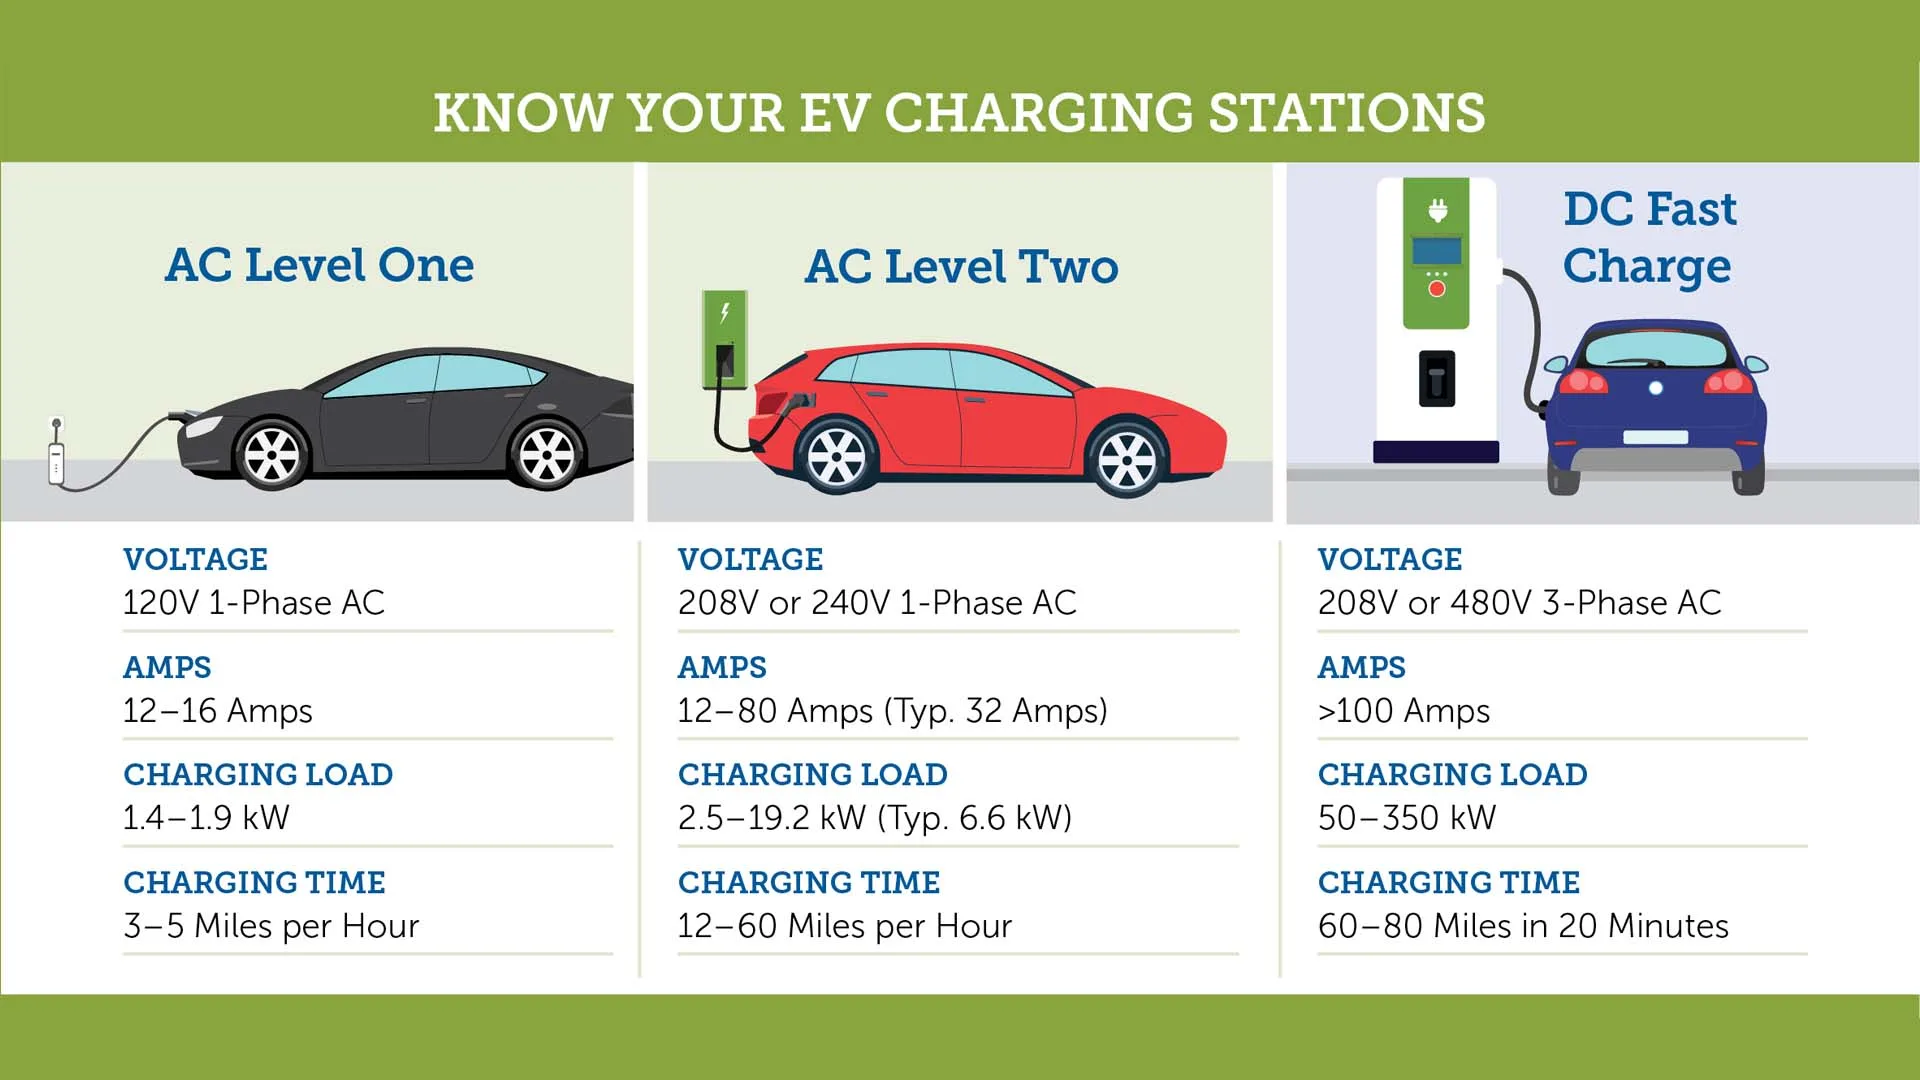
\includegraphics[width=1\textwidth]{images/EVCharger-Levels-jpg.png}
    \centering
    \caption[Typy nabíjania elektromobilov]{Všetky dnešné typy nabíjania elektromobilov s príslušnými údajmi o rýchlosti nabíjania a kapacite kábla. Zdroj obrázka: \cite{websitecharginglevels2023}.}
    \label{typynabijania:obr}
    \end{figure}

    %TODO: lepsie vysvetlit pojmy
% \UNFIN

%TODO specifikovat pre implementaciu, je to v nejakom clanku

% \subsection{Rýchlosť nabíjania batérie.}
% % \subsection{Rýchlosť nabíjania batérie.}
% Pomocou triedy Battery, ktorá definuje ideálny model batérie vieme sami definovať vlastné modely batérie.
% Rýchlosť nabíjania ideálnej batérie je:

% \begin{equation}
%     \hat{r}(t) = min\{\overline{r}, \, r(t), \, \hat{e}(t)\},
% \end{equation}
% kde $\overline{r}$ je maximálna rýchlosť nabíjania, $r(t)$ je pilotový signál poslaný do batérie a $\hat{e}(t)$ je nezaplnená energia batérie v čase $t$ v ampéroch. 

% Existuje aj rozšírenie triedy Battery, ktoré sa nazýva Linear2StageBattery. Linear2StageBattery aproximuje po častiach lineárne nabíjanie elektromobilov s lítiovou batériou. Prvý stav, ktorý nazývame hromadné nabíjanie trvá zvyčajne od 0 do 70 až 80 percent stavu nabíjania. Rýchlosť nabíjania batérie Linear2StageBattery je:
% \begin{equation}
%     \hat{r}(t) = 
%     \begin{cases*}
%         min\{\overline{r}, \, r(t), \, \hat{e}(t)\} & Ak $SoC \leq th$ \\
%         min  \{ (1 - SoC) \frac{\overline{r}}{1 - th}, \, r(t) \}      & inak
%     \end{cases*}
%   \end{equation}
% kde $th$ je hodnota energie po prechode z hromadného nabíjania do absorpčného nabíjania. Premenná $SoC$ znamená stav nabíjania batérie.

% Tento čiastočný lineárny model je dobrá aproximácia správania batérie počas nabíjania. Žiaľ, ani tento model nezachytáva všetky prípady, ktoré môžu správanie batérie zmeniť. \cite{lee2021acnsim}

\subsection{Infraštruktúra nabíjacej stanice.}
% \subsection{Typy nabíjacích staníc}

Simulátor ACN-Sim využíva inštancie triedy ChargingNetwork na modelovanie infraštruktúry nabíjacej siete. To znamená, že trieda ChargingNetwork modeluje nabíjačky (napríklad ich počet, typ nabíjačiek atď), transformátor (určený na prenos energie v nabíjacej sieti), prepínacie panely a káble. 

Na zmenu alebo rozšírenie funkcionality triedy ChargingNetwork je nutné vytvoriť novú triedu, ktorá dedí od triedy ChargingNetwork. Takto bola vytvorená trieda StochasticNetwork, ktorá sa odlišuje od triedy ChargingNetwork v prideľovaní nabíjačiek prichádzajúcim elektromobilom. Popis, ako sa prideľujú nabíjačky elektromobilom:
% upravit poslednu vetu 

%pouzivat nabijacia siet 
% Typy nabíjacích staníc (implementované v balíku acnportal), ktoré pri experimentoch využívame sú:

\subsubsection*{ChargingNetwork} V tomto type nabíjacej siete je každý prichádzajúci elektromobil priradený vopred priradený určenej nabíjačke v nabíjacej sieti. 

\subsubsection*{StochasticNetwork} Tento typ nabíjacej siete prideľuje každému prichádzajúcemu elektromobilu voľnú nabíjačku náhodne. V prípade, keď príde elektromobil do nabíjacej stanice a žiadna nabíjačka v nabíjacej stanici nie je voľná, tak elektromobil pridá do na koniec čakacieho radu. Potom v okamihu, keď sa nabíjačka uvoľní, tak sa priradí prvému elektromobilu v čakaciom rade (ktoré sa z čakacieho radu odstráni).   \\



% druha vec netreba, lebo tu nechceme 
%

% Táto nabíjacia stanica prideľuje nabíjačky elektromobilom náhodne. Implementuje čakací front v prípade ak nie sú voľné nabíjačky. 
% Ak nastavíme parameter early departure na pravdivý, tak dovolíme výmenu vozidla nabíjajúcim na stanici s vozidlom, ktoré sa nachádza v čakacom fronte. 

Typ nabíjacej siete StochasticNetwork je viac vhodný než typ nabijacej siete ChargingNetwork hlavne pre uplatnenie v praxi, ale aj v pri generovaní udalostí zo štatistických modelov. \cite{lee2021acnsim}

Keďže my chceme, aby naše experimenty boli aplikovateľné v reálnom živote, tak používame typ siete StochasticNetwork v experimentoch. Tiež používame v našim experimentoch len nabíjačky, ktoré povoľujú prenos akéhokoľvek množstva energie medzi dolnou a hornou hranicou množstva energie.
%TODO: zmenit opis lebo oni tam pisu ze vseliake typy nabijaciek s obmedzeniami sa vyuziva v realnom zivote
% \UNFIN

\subsection{Obmedzenia pri nabíjaní.}
% \subsection{Obmedzenia pri nabíjaní.}
\label{Vych:konfig:obmedzenia}

Nabíjacie systémy často fungujú na princípe radiálnych sietí. Musíme preto obmedziť množstvo voltov prechádzajúcich cez každé úzke miesto siete. Pomocou Kirchhoffových zákonov vieme definovať obmedzenia pri nabíjaní takto: 
% V radialných sieťach dostávajú elektrické autá energiu prostredníctvom jediného zdroja. ... 

\begin{equation}\label{eq:current}
    |I_{j}(t)| = |\sum_{i=1}^{N} \, A_{ij} \, r_{i} (t) \,e^{j\phi_{i}}| \leq R_{j},
\end{equation}
kde $R_{j}$ je veľkosť prúdu, $I_{j}(t)$ je prúd prúdiaci cez úzke miesto siete, $N$ je počet nabíjačiek v nabíjacej stanici, $r_{i}(t)$ je prúd poskytovaný nabíjačkou $i$ v čase $t$. Dokopy máme $T$ časových krokov. Parametrom $\phi_{i}$ vyjadrujeme fázový uhol pre aktuálny fázor, ktorý závisí na tom ako je nabíjačka $i$ zapojená do siete. \cite{lee2021acnsim}  % v čase $t$ \\

\UNFIN


%TODO: mozno pridat aj dalsi typ obmedzeni spominany v jednom z clankov?


\section{Prvý experiment}



\section{Druhý experiment}




\section{Tretí experiment}




